\documentclass{article}

% Package necessari
\usepackage[a4paper]{geometry}
\usepackage[utf8]{inputenc}
\usepackage[italian]{babel}
\usepackage[T1]{fontenc}
\usepackage[font={small,sl}]{caption}
\usepackage[font={small,sl}]{subcaption}
\usepackage{graphicx}
\usepackage[usenames, table, dvipsnames]{xcolor}
\usepackage{hyperref}
\usepackage[most]{tcolorbox}
\usepackage[section]{placeins}
\usepackage{soulutf8}
\usepackage{listings}
\usepackage{tabularray}

% Titolo del documento
\title{\small Relazione del progetto di Sistemi Operativi Avanzati \\
\Huge \textbf{Multi-flow Device File}}

% Autore del documento
\author{Simone Tiberi (M. 0299908)\\%
(email: \texttt{\href{mailto:simone.tiberi.98@gmail.com}{simone.tiberi.98@gmail.com}})}

% Data del documento
\date{\today}

% Impostazione delle lunghezze di alcuni elementi del documento
\setlength{\parskip}{1em}
\setlength{\parindent}{0em}

% Impostazioni del package hyperref
\hypersetup{
        colorlinks=true,
        linktocpage=true,
        linkcolor=blue,
        urlcolor=blue,
        pdftitle={Relazione progetto SOA},
        pdfauthor={Simone Tiberi},
}

% Tokyonight colors
\definecolor{tn-bg}{HTML}{24283b}
\definecolor{tn-terminal}{HTML}{414868}
\definecolor{tn-red}{HTML}{f7768e}
\definecolor{tn-fg}{HTML}{c0caf5}
\definecolor{tn-fg-dark}{HTML}{a9b1d6}
\definecolor{tn-green}{HTML}{9ece6a}
\definecolor{tn-comment}{HTML}{565f89}
\definecolor{tn-blue0}{HTML}{3d59a1}
\definecolor{tn-blue}{HTML}{7aa2f7}
\definecolor{tn-cyan}{HTML}{7dcfff}

\lstset{
	language=C,
	frame=shadowbox,
        backgroundcolor=\color{tn-bg},
	rulesepcolor=\color{tn-terminal},
        basicstyle=\color{tn-fg}\ttfamily\scriptsize,
	keywordstyle=\color{tn-red}\bfseries\scriptsize,
	stringstyle=\color{tn-green}\scriptsize,
	commentstyle=\color{tn-comment}\scriptsize,
	numbers=left,
	numberstyle=\tiny\color{tn-fg-dark},
	numbersep=5pt,
	tabsize=2,
	showtabs=false,
	showspaces=false,
	showstringspaces=false,
	escapechar=|,
	captionpos=b,
	breaklines=true,
	keepspaces=true
}

\renewcommand{\lstlistingname}{Listato}
\graphicspath{ {./figs/} }

\newtcolorbox{custombox}[1]{
        colframe = blue!25,
        colback  = blue!10,
        coltitle = blue!20!black,
        title    = #1,
        breakable,
        enhanced,
}

% Tabelle
\renewcommand{\arraystretch}{1.5}
\setlength{\arrayrulewidth}{0.1em}

\newcommand{\terminal}[1]{\colorbox{tn-bg}{\textcolor{tn-fg}{\texttt{#1}}}}

\begin{document}
\maketitle

\section{Specifica del progetto (traduzione)}
La specifica richiede l'implementazione di un device driver Linux per la gestione di flussi di dati a due livelli di priorità. Attraverso una sessione aperta verso un dispositivo, un thread può leggere/scrivere dati in modo tale che:
\begin{itemize}
        \item la consegna dei dati segua una politica \textbf{FIFO} (\textbf{F}irst-\textbf{I}n-\textbf{F}irst-\textbf{O}ut),
        \item non appena letti, i dati \textbf{scompaiano} dal flusso,
        \item la scrittura sul flusso ad alta priorità sia \textbf{sincrona},
        \item la scrittura sul flusso a bassa priorità sia \textbf{asincrona}, basata su deferred work, \ul{mantenendo comunque la sincronia nella notifica dell'esito dell'operazione} (in conformità all'interfaccia della \texttt{write}),
        \item la scrittura sia sempre eseguita in modo sincrono,
        \item il driver supporti al più \textbf{128} devices associati al corrispettivo minor number.
\end{itemize}

Il device driver deve implementare il supporto all'operazione \texttt{ioctl}, al fine di gestire le sessioni di I/O e permettere:
\begin{itemize}
        \item di impostare il livello di priorità (\texttt{HIGH} or \texttt{LOW}) per le operazioni,
        \item di scegliere se effettuare letture e/o scritture in modo bloccante o meno,
        \item di impostare un timeout per regolare il risveglio in caso di richieste bloccanti.
\end{itemize}

Inoltre è richiesto di implementare un meccanismo per abilitare o disabilitare i dispositivi in termini di minor numbers, basato sui parametri del modulo. Nel caso in cui un dispositivo sia disabilitato, ogni tentativo di apertura di nuova sessione deve fallire, ma devono comunque continuare ad essere gestite quelle aperte in precedenza.

Altri parametri addizionali esposti tramite VFS devono fornire un'immagine dello stato corrente dei device in termini di:
\begin{itemize}
        \item abilitazione,
        \item numero di byte correntemente presenti nei due flussi,
        \item numero di thread correntemente in attesa nei due flussi.
\end{itemize}

\section{Struttura del repository}
La realizzazione della specifica è stata organizzata, all'interno del repository, nelle seguenti cartelle:
\begin{itemize}
        \item nella radice è presente uno script \texttt{bash} per la creazione di nodi di I/O pilotabili con il driver sviluppato,
        \item in \texttt{KERNEL\_MODULE/} è contenuto il codice effettivo del driver,
        \item in \texttt{USER\_LIB/} è contenuta una libreria utente per facilitare l'interfacciamento con i nodi di I/O associati al driver sviluppato,
        \item in \texttt{SAMPLES/} sono presenti una semplice demo e un file contenente diversi test cases.
\end{itemize}

\section{Driver per la gestione dei dispositivi multi-flusso}
\begin{figure}[htbp]
        \centering
        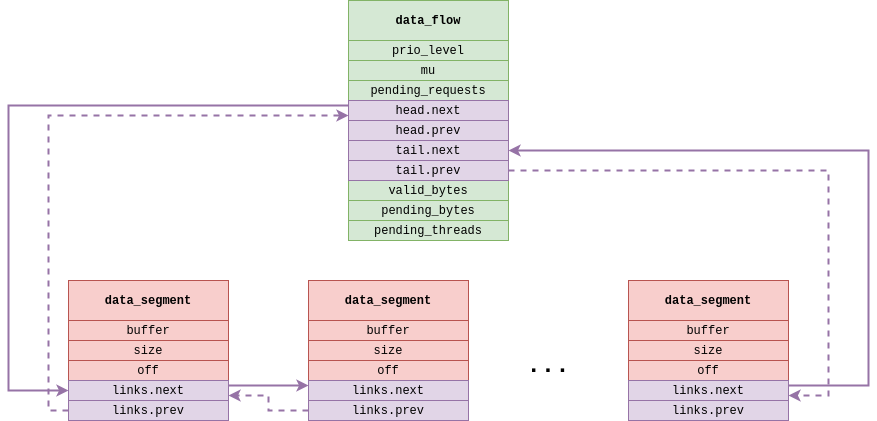
\includegraphics[width=.8\textwidth]{data}
        \caption{Gestione dei dati all'interno dei vari devices}
        \label{fig:data}
\end{figure}

In fig. \ref{fig:data} è riportato uno schema dell'architettura adottata, all'interno della soluzione proposta, per la gestione dei dati. Una delle strutture adottate, per la realizzazione dell'implementazione, è la \texttt{data\_flow}, la quale rappresenta il singolo flusso di dati associato ad un device.

In essa sono presenti:
\begin{itemize}
        \item il livello di priorità (\texttt{HIGH\_PRIO} o \texttt{LOW\_PRIO}) a cui il flusso è associato,
        \item il mutex per garantire l'atomicità nell'aggiornamento delle strutture dati necessarie alla gestione del flusso di dati,
        \item la wait queue dove i thread possono attendere nel caso in cui le loro richieste bloccanti non siano momentaneamente soddisfacibili,
        \item la testa e la coda di una lista collegata per l'effettiva memorizzazione dei dati, il cui meccanismo di collegamento è esemplificato in fig. \ref{fig:data},
        \item il numero di byte \textit{validi}, ovvero scritti ma non ancora letti,
        \item il numero di byte \textit{pendenti}, ovvero accettati come deferred work, ma non ancora effettivamente scritti nel flusso,
        \item il numero di thread in attesa della disponibilità di dati da leggere o di spazio utilizzabile in scrittura.
\end{itemize}

Un ulteriore struttura presente in fig. \ref{fig:data} è la \texttt{data\_segment}, la quale rappresenta il chunk di dati scritto sul flusso da una singola operazione di scrittura. Per questo motivo al suo interno sono presenti:
\begin{itemize}
        \item il buffer effettivo in cui memorizzare i dati scritti,
        \item la taglia complessiva dei dati scritti dall'operazione,
        \item l'offset a cui iniziare a leggere i dati,
        \item una coppia di pointers (\texttt{struct list\_head}) per il collegamento con gli altri chunks.
\end{itemize}

Dalla specifica si evince come ogni device $i$ (con $0\leq i \leq 127$) debba supportare due flussi di dati associati a priorità distinte e che la selezione del livello su cui effettuare le operazioni sia \textbf{per sessione}, per cui in fig. \ref{fig:get_active_flow} è riportato lo schema della soluzione scelta per implementare questa meccanica.

\begin{figure}[htbp]
        \centering
        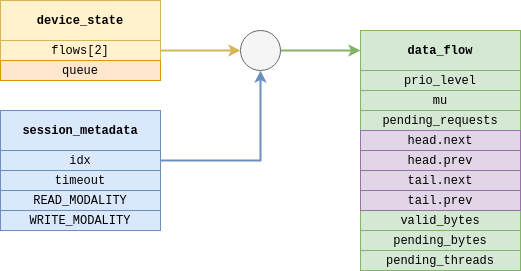
\includegraphics[width=.8\textwidth]{get_active_flow}
        \caption{Come reperire il flusso attualmente attivo a partire dalla sessione}
        \label{fig:get_active_flow}
\end{figure}

In particolare in essa sono compaiono altre due nuove strutture:
\begin{itemize}
        \item la \texttt{device\_state}, in cui sono contenuti i metadati associati al dispositivo, quali:
                \begin{itemize}
                        \item il vettore dei due flussi di dati,
                        \item la work queue in cui accodare le scritture \texttt{LOW\_PRIO} che debbono essere gestite in modo deferred;
                \end{itemize}
        \item la \texttt{session\_metadata} che raccoglie al suo interno il set minimale di informazioni necessarie per la gestione della sessione aperta verso un device, ovvero:
                \begin{itemize}
                        \item l'indice necessario al fine di spiazzarsi all'interno dell'array di flussi contenuto nella struttura \texttt{device\_state},
                        \item il timeout da utilizzare nel caso in cui si deve attendere per dati da leggere o spazio utilizzabile in scrittura,
                        \item le modalità, bloccanti o meno, di lettura e scrittura.
                \end{itemize}
\end{itemize}

È opportuno osservare che tutti i campi della struttura \texttt{session\_metadata} vengono acceduti atomicamente, o perché definiti come \texttt{atomic[\_long]\_t}, o perché sono singoli bit.

In definitiva dunque l'iter per reperire il riferimento al flusso corrente adottato in tutta l'implementazione, attraverso la macro \texttt{get\_active\_flow}, è il seguente:
\begin{enumerate}
        \item si accede all'array globale \texttt{struct device\_state devs[MINORS]} utilizzando il minor number come indice. Questo viene reperito in modalità differenti a seconda della versione del kernel Linux in esercizio, sfruttando una macro apposita;
        \item si preleva dalla sessione l'indice di priorità attualmente configurato e lo si usa per spiazzarsi all'interno dell'array \texttt{flows}.
\end{enumerate}

\subsection{File operations}
\subsubsection{Apertura della sessione (\texttt{open})}
La \texttt{mfdf\_open}, ovvero l'implementazione all'interno del driver dell'operazione di apertura è molto semplice e si limita a:
\begin{itemize}
        \item verificare se il dispositivo è correntemente abilitato, ed in caso contrario restituire il codice d'errore \texttt{EAGAIN} al chiamante,
        \item allocare, mediante \texttt{SLAB} allocator, una struttura \texttt{session\_metadata} descritta poc'anzi e collegarla alla \texttt{struct file} sfruttando l'apposito pointer generico \texttt{private\_data},
        \item inizializzare i campi della sessione a valori di default (e.g. flusso attivo: \texttt{LOW\_PRIO}).
\end{itemize}

\subsubsection{Rilascio della sessione (\texttt{release})}
La \texttt{mfdf\_release}, ovvero l'implementazione all'interno del driver dell'operazione di rilascio, essendo duale dell'apertura, si limita a liberare il buffer allocato per la memorizzazione dei metadati relativi alla sessione.

\subsubsection{Scrittura (\texttt{write})}
Nella \texttt{mfdf\_write}, ovvero l'implementazione all'interno del driver dell'operazione di scrittura, per prima cosa si \textit{pre-alloca} la struttura \texttt{data\_segment} in cui scrivere i dati richiesti, per minimizzare la dimensione della sezione critica. È opportuno osservare che in funzione della modalità di scrittura selezionata nella sessione vengono impostati i flag per la richiesta di memoria (\texttt{GFP\_ATOMIC} o \texttt{GFP\_KERNEL}).

Si passa poi ad eseguire un blocco di codice responsabile di mandare eventualmente \textit{a dormire} i thread che effettuano richieste bloccanti non soddisfacibili. L'iter seguito è il seguente:
\begin{enumerate}
        \item si incrementa atomicamente il numero di thread pendenti,
        \item si passa allo stato \texttt{TASK\_INTERRUPTIBLE} tramite la \texttt{wait\_event\_interruptible\_timeout}. Il controllo per il risveglio viene effettuato invocando una funzione che:\begin{enumerate}
                \item tenta di prendere il lock,
                \item effettua il controllo,
                \item in caso positivo ritorna \texttt{TRUE} \textbf{senza rilasciare il lock}\footnote{Questo garantisce che una volta ripreso il controllo, in caso di successo dell'API nessuno può aver modificato lo stato del flusso.} altrimenti rilascia il lock e torna \texttt{FALSE}
        \end{enumerate}
        \item si decrementa atomicamente il numero di thread pendenti,
        \item eventualmente si ritorna al chiamante restituendo come codici d'errore:
                \begin{itemize}
                        \item \texttt{ETIME} nel caso in cui la richiesta non è stata soddisfatta nel timeout settato,
                        \item \texttt{EINTR} nel caso in cui il thread è stato colpito da segnale.
                \end{itemize}
\end{enumerate}

Dopodiché si effettua realmente la scrittura:
\begin{itemize}
        \item nel caso \texttt{HIGH\_PRIO}, semplicemente invocando la funzione responsabile di effettuare il collegamento delle strutture dati come mostrato in fig. \ref{fig:data},
        \item nel caso \texttt{LOW\_PRIO} schedulando il deferred work. A tal proposito in fig. \ref{fig:deferred_work} è riportata la relazione che sussiste fra le strutture in gioco.
\end{itemize}

A livello implementativo, è stato scelto di utilizzare una work queue privata \textit{single threaded} per garantire l'ordinamento FIFO. Questo perché la linearizzazione temporale delle scritture del buffer avviene prendendo come punto di riferimento l'istante di inserimento in coda (i.e. non è possibile che se il thread $T_1$ inserisce in coda una scrittura \textbf{prima} del thread $T_2$, questa venga effettivamente scritta sul flusso \textbf{prima} della precedente).

L'allocazione delle code \textit{single threaded} è stata realizzata in modo differente a seconda della versione del kernel Linux correntemente in esercizio:
\begin{itemize}
        \item tramite la \texttt{alloc\_ordered\_workqueue} dalla versione \texttt{2.6.36}, ovvero con l'avvento delle \textbf{CMWQ} (\textbf{C}oncurrency \textbf{M}anaged \textbf{W}ork\textbf{Q}ueue),
        \item tramite la \texttt{create\_single\_threaded\_workqueue} viceversa
\end{itemize}

\begin{figure}[htbp]
        \centering
        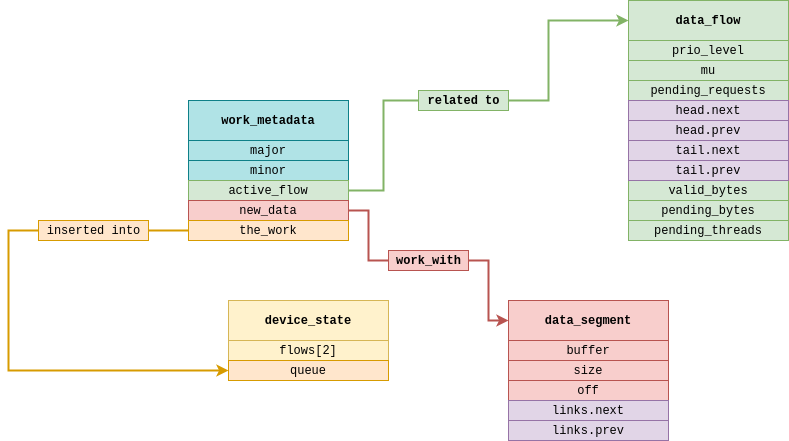
\includegraphics[width=.8\textwidth]{deferred_work}
        \caption{Relazione delle strutture coinvolte nel meccanismo del deferred work}
        \label{fig:deferred_work}
\end{figure}

Relativamente al deferred work, è opportuno analizzare l'uso del campo \texttt{pending\_bytes}. L'idea è quella di garantire che il valore restituito all'utente in modo sincrono sia effettivamente pari al numero di bytes scritti nel flusso in modo deferred.

Per garantire ciò ogni qualvolta si verifica l'effettiva disponibilità di spazio scrivibile, nel caso \texttt{LOW\_PRIO} si tiene conto anche dei byte che sono stati già presi in carico, ma non sono ancora stati scritti, ovvero i \texttt{pending\_bytes}.

Infine, prima di ritornare al chiamante, si invoca una \texttt{wake\_up\_interruptible} per risvegliare i thread in attesa. La scelta implementativa è stata quella di adottare una coda singola \textbf{per flusso}, in cui dunque confluiscono sia lettori che scrittori. Analizzando i possibili scenari è facile accorgersi che nella maggior parte dei casi in coda o vi sono soltanto readers o soltanto writers.

L'unica alternativa a ciò, si verifica in casi \textit{transienti} come la timeline di seguito riportata:
\begin{enumerate}
        \item il flusso è saturo,
        \item arriva una richiesta di scrittura bloccante da parte del thread $X$ che lo porta nello stato di \texttt{TASK\_INTERRUPTIBLE},
        \item arriva una richiesta di lettura da parte del thread $Y$ di un numero di byte pari alla taglia massima del flusso di dati,
        \item \ul{prima che lo scrittore venga risvegliato}, arriva un'ulteriore richiesta di lettura da parte del thread $Z$, che lo porta nello stato di \texttt{TASK\_INTERRUPTIBLE}.
\end{enumerate}

\subsubsection{Lettura (\texttt{read})}
Nella \texttt{mfdf\_read}, ovvero l'implementazione all'interno del driver dell'operazione di lettura, per prima cosa si entra all'interno del blocco di codice responsabile eventualmente di \textit{mandare a dormire} il thread richiedente, del tutto equivalente a quello descritto per la \texttt{mfdf\_write}.

Si invoca poi una funzione responsabile di realizzare l'effettiva lettura dei dati dalla lista di strutture \texttt{data\_segment} collegate al flusso.

L'idea in questo caso è quella di leggere a partire da \texttt{head->next}, ovvero il primo \texttt{data\_segment} associato al flusso, fintantoché non si arriva alla \texttt{tail} e, ad ogni iterazione:
\begin{enumerate}
        \item computare i byte effettivamente leggibili come $\min\lbrace\Delta_{tot}, \Delta_{segment}\rbrace$, dove:
                \begin{itemize}
                        \item $\Delta_{tot}$ corrisponde alla differenza tra quanto è stato richiesto di leggere e quanto è stato già letto,
                        \item $\Delta_{segment}$ corrisponde alla differenza tra la taglia complessiva dei dati contenuti in $segment$ e quanti byte sono stati già letti da esso per via di letture precedenti;
                \end{itemize}
        \item copiare i byte all'interno del buffer specificato dall'utente, aggiornando il numero totale di byte letti e l'offset del segmento corrente,
        \item nel caso in cui siano stati letti tutti i byte nel segmento, procedere a scollegarlo dalla lista, facendo dunque puntare la testa all'elemento successivo.
\end{enumerate}

Infine si risvegliano i thread in coda prima di restituire il numero di byte letti al chiamante.
\subsubsection{Configurazione della sessione (\texttt{ioctl})}
La \texttt{mfdf\_ioctl} è caratterizzata da un prototipo condizionale all'interno dell'implementazione. Questo perché dalla versione \texttt{2.6.35} la \texttt{ioctl} è stata rimossa in favore di due alternative:
\begin{itemize}
        \item \st{\texttt{compat\_ioctl}} per la compatibilità con i programmi utente a 32 bit,
        \item \ul{\texttt{unlocked\_ioctl}} che, a differenza della \textit{vecchia} \texttt{ioctl}, \textbf{non prende il BKL} (\textbf{B}ig \textbf{K}ernel \textbf{L}ock).
\end{itemize}

A livello di prototipo, la versione \texttt{unlocked} e quella tradizionale differiscono per la presenza di un pointer all'\texttt{inode} nella firma, che comunque non viene utilizzato. Per questo motivo l'uso del costrutto \texttt{\#ifdef\dots\#endif} è limitato alla sola firma.

A livello implementativo, la funzione presenta uno switch-case in cui, in base al \texttt{cmd} passato, vengono impostati i diversi campi della struttura \texttt{session\_metadata}, previa aver sanitizzato l'\texttt{arg} passato.

Per evitare di utilizzare come \texttt{cmd} codici \textit{well-known} è stata adottata la macro \texttt{\_IOW}, definita all'interno dell'header file \texttt{linux/ioctl.h}, la quale genera l'operational code a partire da:
\begin{itemize}
        \item un \textit{magic number} unico in tutto il kernel,
        \item un codice effettivo unico all'interno del driver.
\end{itemize}

\subsection{Parametri del modulo}
All'interno del VFS \texttt{sys} sono esposte diverse informazioni associate all'operatività del driver:
\begin{itemize}
        \item il valore del major number, utile per lo script di generazione di nodi e per la fase di testing (read only),
        \item l'array dei flag di abilitazione dei devices (read/write),
        \item il numero di byte standing nei due flussi per ogni dispositivo (read only),
        \item il numero di byte standing threads nei due flussi per ogni dispositivo (read only).
\end{itemize}

In particolare, per evitare che il major number venga modificato in maniera illegittima (e.g. cambiando manualmente i privilegi associati al file), anziché adottare la macro \texttt{module\_param} è stata utilizzata la versione con il callback esplicito, andando a porre come operazione \texttt{set} \texttt{NULL}.

Per quanto riguarda invece gli ultimi due punti dell'elenco precedente, la strategia adottata è stata differente. Anziché estrarre dalle strutture dati i campi ed utilizzare array globali, è stato preferito utilizzare \texttt{kobjects} e \texttt{kobj\_attribute}, per esporre informazioni intrinsecamente read only e mantenere dunque i vari metadati raggruppati in modo semanticamente significativo.

Per cui è stato creato un nuovo kernel object \texttt{mfdf} all'interno della directory \texttt{/sys/kernel}, a cui sono stati associati due attributi, ovvero \texttt{standing\_bytes} e \texttt{standing\_threads}.

In definitiva dunque in tabella \ref{table:params} è riportata una sintesi di \textit{dove} e \textit{come} consultare le informazioni esposte tramite \texttt{sys}.

\begin{table}[htbp]
        \centering
        \begin{tblr}{
                colspec = {|l|l|l|},
                hlines,
                row{odd} = {tn-blue},
                row{even} = {tn-cyan},
                row{1} = {tn-blue0,font=\bfseries\color{white}},
        }
        Informazione & Pseudofile & Permessi\\
        Abilitazione dispositivi & \texttt{/sys/module/mfdf/parameters/enable} & \texttt{0660}\\
        Major ottenuto dalla registrazione & \texttt{/sys/module/mfdf/parameters/major} & \texttt{0440}\\
        Byte standing per dispositivo & \texttt{/sys/kernel/mfdf/standing\_bytes} & \texttt{0440}\\
        Thread standing per dispositivo & \texttt{/sys/kernel/mfdf/standing\_threads} & \texttt{0440}\\
        \end{tblr}
        \caption{Informazioni esposte in \texttt{sys}}
        \label{table:params}
\end{table}

\subsection{Installazione del modulo}
Per installare il modulo kernel è possibile utilizzare le regole specificate all'interno del \texttt{Makefile}:
\begin{itemize}
        \item \terminal{\$ make} compila il modulo, utilizzando la regola \texttt{make modules} di \texttt{kbuild},
        \item \terminal{\# make install} monta il modulo, tramite \texttt{insmod}, ed installa l'header file necessario per l'utilizzo dell'\texttt{ioctl} \textit{user-level} in \texttt{/usr/local/include/mfdf},
        \item \terminal{\$ make clean} rimuove l'output della compilazione dalla directory locale,
        \item \terminal{\# make clean-all} in più al semplice \texttt{clean}:
                \begin{itemize}
                        \item smonta il modulo, se questo è effettivamente montato, sfruttando un costrutto condizionale per evitare errori,
                        \item rimuove l'header file \texttt{/usr/local/include/mfdf/ioctl.h}.
                \end{itemize}
\end{itemize}

\section{Libreria utente}
La libreria utente è costituita da una serie di ridefinizioni, tramite direttive \texttt{\#define}, di alcune funzioni tipiche delle librerie \texttt{fcntl.h} e \texttt{unistd.h} tipiche per la gestione di oggetti di I/O (e.g. \texttt{open}, \texttt{write}, \dots).

L'unica funzione effettivamente realizzata \textit{ex-novo} è un wrapper della write, per poter formattare il \textit{cosa} scrivere secondo una regola \texttt{printf}-like.

Relativamente al Makefile presente nella directory, tramite la regola:
\begin{itemize}
        \item \terminal{\$ make} è possibile compilare la libreria utente e generare:
                \begin{itemize}
                        \item il file oggetto (\texttt{user.o}),
                        \item l'archivio utilizzabile dal linker (\texttt{libmfdfuser.a});
                \end{itemize}
        \item \terminal{\$ make doc} è possibile convertire il file markdown contenente il manuale della libreria utente nel formato delle manpages;
        \item \terminal{\# make install} è possibile:
                \begin{itemize}
                        \item installare l'header file, contenente le direttive \texttt{\#define} ed il prototipo della funzione \texttt{printf}-like sopra citate, all'interno della directory \texttt{/usr/local/include/mfdf},
                        \item installare la libreria statica \texttt{libmfdfuser.a} all'interno della directory \texttt{/usr/local/lib/mfdf},
                        \item comprimere, utilizzando \texttt{gunzip}, la manpage generata dalla regola \texttt{doc},
                        \item installare la manpage compressa all'interno della directory \texttt{/usr/local/share/man/man0p};
                \end{itemize}
        \item \terminal{\$ make clean} è possibile rimuovere dalla directory locale ogni output prodotto dalle regole descritte in precedenza;
        \item \terminal{\# make clean-all} è possibile rimuovere anche gli output installati nelle directory globali.
\end{itemize}

In definitiva dunque, per maggiori informazioni relativamente all'utilizzo della libreria è possibile:
\begin{itemize}
        \item installarla, utilizzando il comando \terminal{\$ make \&\& make doc \&\& sudo make install},
        \item consultare la pagina di manuale utilizzando il comando \terminal{\$ man mfdf\_user.h}
\end{itemize}

Un esempio di utilizzo della libreria utente è riportato nel listato \ref{lst:demo}, compilabile utilizzando come flags:
\begin{itemize}
        \item \texttt{-L/usr/local/lib/mfdf} per aggiungere la directory a quelle ispezionate di default per individuare le libreria da linkare,
        \item \texttt{-lmfdfuser} per linkare effettivamente la libreria.
\end{itemize}

\section{Testing del modulo}
Per testare il corretto funzionamento del modulo è stato utilizzato il file \texttt{SAMPLES/src/test-cases.c}. L'idea è stata quella di definire una struttura che rappresentasse il caso di test, ovvero la \texttt{struct test\_case} i cui campi sono:
\begin{itemize}
        \item il nome del test, utile per l'attività di auditing,
        \item il function pointer della routine di test, del tipo \texttt{void T(int, int)}.
\end{itemize}

Per cui all'interno del \texttt{main} non si fa altro che:
\begin{enumerate}
        \item reperire il minor number, leggendolo tramite funzione apposita da \texttt{/sys},
        \item invocare, per ogni entry dell'array \texttt{test\_cases} (list: \ref{lst:test-cases}), la funzione \texttt{do\_test} responsabile:
                \begin{itemize}
                        \item dell'inizializzazione dell'ambiente,
                        \item del cleanup dell'ambiente,
                        \item della stampa dei risultati.
                \end{itemize}
\end{enumerate}

In compilazione, è possibile abilitare o meno la modalità \texttt{VERBOSE} al fine di mostrare, per ciascun caso di test, \textit{expected} e \textit{actual values}, mediante il comando \terminal{\$ make MORE\_FLAGS=-DVERBOSE}.

\appendix
\section{Codici citati all'interno del report}
\lstinputlisting[
	caption={File: demo.c},
	label={lst:demo},
	escapechar=
]{../SAMPLES/src/demo.c}

\newpage
\lstinputlisting[
        caption={Test cases realizzati},
	label={lst:test-cases},
	escapechar=,
        firstline=472,
        lastline=494
]{../SAMPLES/src/test-cases.c}

\end{document}
